% Chapters are the next main unit.
\chapter{Introduction}
\label{chp:intro}

We begin this chapter by introducing robotic manipulation using force and tactile sensors, and present the challenges in programming robots to perform manipulation tasks in the physical world.
Following this, we state the specific problem we wish to address in this thesis as well as the motivations behind seeking its solution.
The chapter concludes with main contributions and thesis structure.

%%%%%%%%%%%%%%

\section{Learning to interact with the real world}

Our world is infinitely complex.
%; a setting in which developing complete models, i.e. all rules which govern all things, is infeasible.
By the second law of thermodynamics, any real-world system constantly changes as energy transfers between its composing particles of matter \cite{zubarev1974nonequilibrium}. 
Thus, if one's goal is to interact with such a dynamic ever-changing world, one needs to continually infer relevant truths which exist in that world through some form of external sensing.

This type of approach to system identification and control is known as \emph{model-free} \cite{Spall1998} in the sense that one functions without needing explicit knowledge of physics.

Living organisms are known to take this approach \cite{dayan2008decision}. %when interacting with the real world.
A child does not learn to walk given absolute knowledge of the dynamics which govern his interaction with the environment. Rather, he must build an action-consequence model of the walking task through much trial and error.

By learning a model which maps sensory information to relevant properties of an environment, the entity also gains an ability to predict anomalies.
% within its environment.
Novel events are important as they present opportunities to gain deeper insight into the true underlying principles which define the environment not presently described by the current model.

Humans, who are among the most successful of living organisms, have the ability to both model their environment and efficiently perform inference on that model using their available senses.
For a trained athlete to succeed in the game of basketball, she must learn to ignore irrelevant sensory data, such as the cheering of the crowd, and focus on more important information, such as the image of the basket on her retina.
How can she identify relevant information with respect to her current task?
We are interested in exploring how humans might accomplish this by enabling robots to possess such a skill.

%Consider the following example, a robot might lift a mass of 1kg on multiple occasions and each time experience an identical input pattern across its joint-torque sensors.
%We would like the robot to have the capacity to recognize and associate this pattern with picking up arbitrary objects of mass 1kg.
%Taking this a step further, the robot should be able to exploit the data-driven model it develops in order to guess the mass of a 5kg, 10kg or 20kg object, for example.

%%%%%%%%%%%%%%%%

\section{Problem Statement}

We wish to address the problem of supporting robotic manipulation by efficiently predicting properties of an environment using unlabeled sensory data.
The ability to predict properties of an environment, such as the mass of an object on a table, is an important prelude to closing the loop and allowing robots to adapt to unexpected change.

One barrier to achieving this goal, however, is that the size of the input space increases with the number of sensor readings available to the system.
This makes making predictions susceptible to Bellman's infamous curse of dimensionality.
We therefore take steps to reduce the number of sensors considered when predicting properties of an environment.

To test our solution, we consider a block topple-slide task (see Figure~\ref{fig:topple}) performed by a robot equipped with force, torque and tactile sensors.
In this task, the end effector of the robot pushes on the side of a foam-encapsulated block, causing it to topple, and then pushes the block back to its starting pose against a wall.
A prescribed joint-angle trajectory to achieve this manipulation task is provided by a human expert through kinesthetic teaching.
%The robot tracks the given trajectory in joint space using a standard computed-torque tracking procedure.
The given example trajectory is assumed to be robust in two ways: repeating the trajectory should cause repeated rotations of the block, and the same trajectory should remain successful when applied to blocks with variations in mass, friction, and compliance. 

%The use of a prescribed manipulation trajectory also implies an approximate correspondence between the current elapsed time within a motion and the phase of the manipulation.

\begin{figure}[]
	\centering
	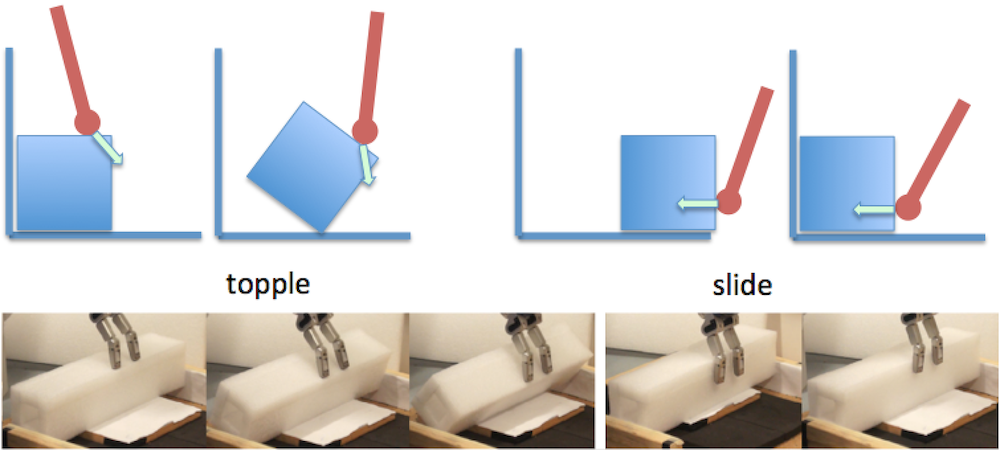
\includegraphics[width=\linewidth]{images/topple}
	\caption{The topple-slide task.}
	\label{fig:topple}
\end{figure}

%%%%%%%%%%%%%%%%%%%

\section{Motivations}
As sensing technologies become more affordable, robots will be able to concurrently make a wide range of measurements within the environments in which they operate.  
As can be seen in Figure~\ref{fig:eg_sensor_trace}, it is clear that sensors with the capacity to measure properties of an environment will obtain distinct readings as those environment properties change. 
Notice how the streams become disjoint during phases of robot-object contacts (during toppling and sliding) and recombine during phases of non-contact.
It then becomes possible, given some form of ground-truth, for the robot to learn a model which explains how changes in its sensor readings relate to changes in its environment.

%Consider a concrete example: the robot may develop a mapping between (1) sensory data traces while handling a piece of fruit and (2) the level of ripeness of the fruit.
%When the robot encounters a piece of fruit that affords a familiar sensory experience (i.e. near previous samples of the sensory input space), the robot has the capacity to classify that piece of fruit as having a particular level of ripeness.

This releases the need for experts to model the relationships between sensory readings and environmental phenomena. 
For example, distinct force measurements may relate to the compliance of an object, which in turn could provide insight into some high-level feature such as its ripeness (if the object were a piece of fruit).
We thereby achieve a highly scalable system capable of mapping arbitrary sensor readings (vision, olfactory, inertial, etc.) to arbitrary environment properties, given the availability of relevant ground-truth information on which to train the model-learning system.

%FIGURE
\begin{figure}[hbt]
	\centering
	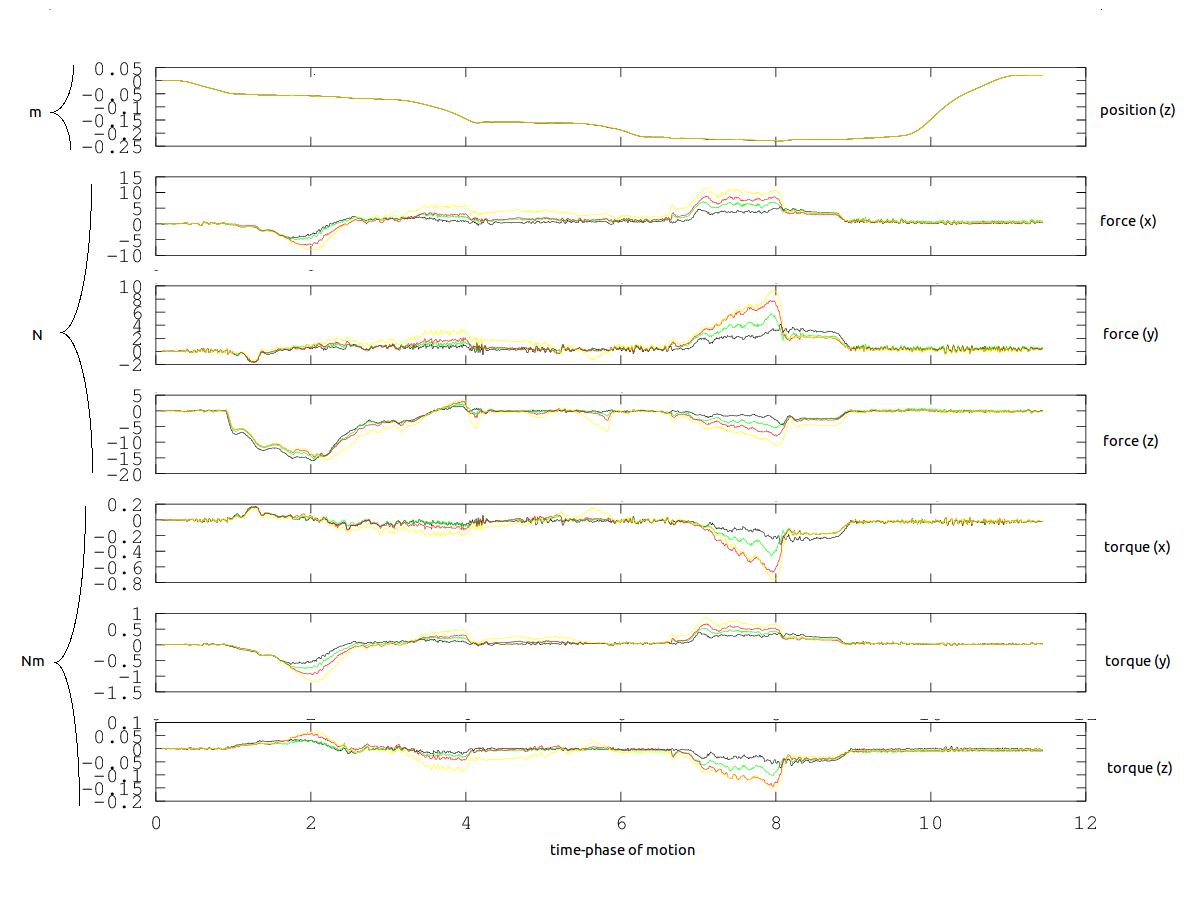
\includegraphics[width=\linewidth]{images/eg_sensor_trace}
	\caption{Example sensory streams during the topple-slide task in different environments (one colour for each environment).
}
	\label{fig:eg_sensor_trace}
\end{figure}
%ENDFIGURE

%%%%%%%%%%%%%%%%%%%



%%%%%%%%%%%%%%%%%%

\section{Contributions}
The contributions of this thesis are three-fold: 
(1) a unifying bridge between literature in robotics, physiology and neuroscience on the topic of exploiting force and tactile sensors for dexterous manipulation, 
(2) an unsupervised feature selection algorithm based on a new metric called the task variance ratio, which filters important sensor readings and motion-phases within high-dimensional sensory data streams during manipulation tasks and 
(3) a supervised learning algorithm with partial least squares (PLS) regression at its core, which builds statistical data-driven models that use important sensory data traces from a robot to predict properties defining its environment.

The feature selection algorithm allows the robot to distinguish between sensors which provide task-critical information, and sensors which provide information that is noisy or irrelevant to the task.
This ability to gauge the usefulness of sensor readings becomes important as the number of sensors in the system increases, and real-time processing of all sensors becomes impossible.
Disregarding all but the most important sensors reduces algorithmic complexity to constant time, which guarantees support for real-time operation irregardless of the number of sensors physically available to the robot.
The developed models are then used to efficiently predict environment properties when novel sensory data traces are recorded by the robot's sensors.

%%%%%%%%%%%%%%%%%%

\section{Thesis Structure}
Following this introductory chapter, we provide background literature on the topic of exploiting force and tactile sensor data for manipulation in the robotics, neuroscience and physiology literature in Chapter~\ref{chap2}.
In Chapter~\ref{chap3}, we more formally define the algorithms and data structures used in our approach.
Chapter~\ref{chap4} contains an overview of the software developed in support of experiments.
In Chapter~\ref{chap5}, we present experimental procedures and results of experiments with the physical robotic system.
Finally, conclusions are drawn in Chapter~\ref{chap6}.
